%! Licence = CC BY-NC-SA 4.0

%! Author = gianfluetsch, mariuszindel
%! Date = 19. Jan 2022
%! Project = pfsec_summary

\section{Betty Bossi}

\begin{center}
    \vspace{-8pt}
    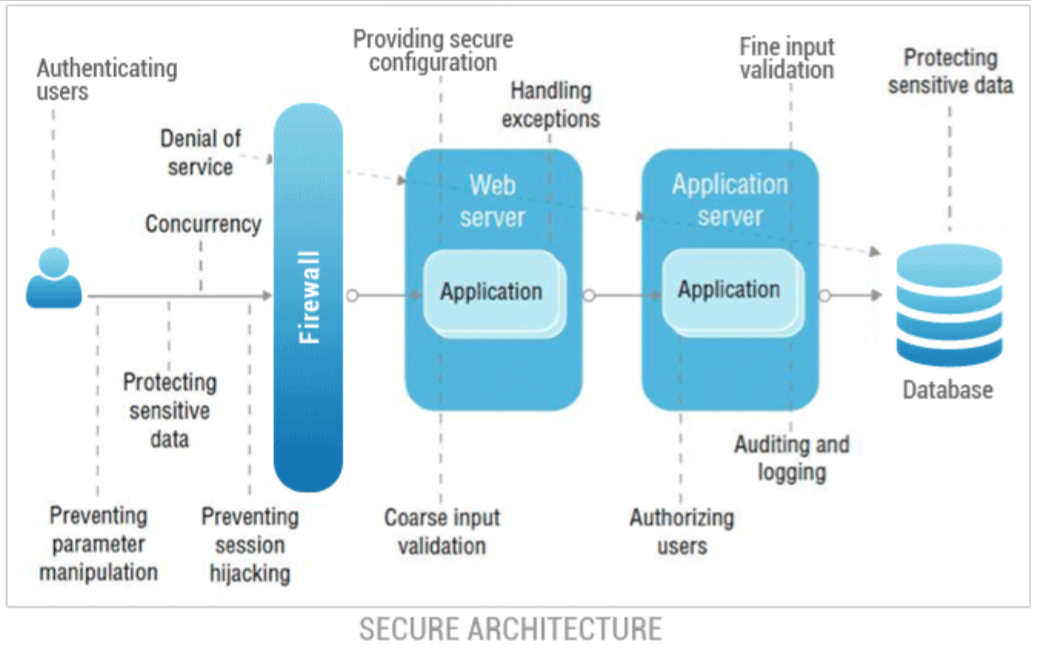
\includegraphics[width=1.0\linewidth]{01-security_components/secure_architecture}
    \vspace{-8pt}
\end{center}

\subsection{Komponente}
\subsubsection{User}
\begin{itemize}
    \item IAM $\rightarrow$ Unternehmen müssen heute auch aus Compliance-Gründen personenbezogene Daten konsistent speichern sowie ständig verfügbar und verlässlich bereithalten
    \item Preventing parameter manipulation (CSRF $\rightarrow$ Cross-Site-Request-Forgery)
    \item Preventing parameter manipulation (MITM $\rightarrow$ Man In The Middle))
\end{itemize}


\subsubsection{External FW}
\begin{itemize}
    \item Preventing DoS attack
    \item Blacklisting IP addresses
    \item Web forensic readiness (Unique ID)
    \item Separating network DMZ / internal / external
    \item WAF
    \item IDS logging / IPS execution
\end{itemize}

\subsubsection{Internal FW}
\begin{itemize}
    \item Separating networks
    \item WAF
    \item IDS logging / IPS execution
\end{itemize}

\subsubsection{Server}
\begin{itemize}
    \item OS security $\rightarrow$ \textit{\nameref{subsec:os-hardening}}
    \item Network security
    \item Access Control of Server itself $\rightarrow$ \textit{\nameref{subsubsec:access-control}}
    \item HW sec?
\end{itemize}

\newpage

\subsection{Keywords - Basic security design principle}
\begin{center}
    \begin{tabular}{l c p{8cm}}
        \hline
        \bfseries{Keyword}                        &    \bfseries{System}              & \bfseries{Description}\\
        \hline\hline
        Economy of mechanism           &   ganzes System        &   KISS\\\hline
        Fail-safe defaults             &   Applikation          &   Access Decision sollte bei Fehler in Safe\-State fallen\\\hline
        Complete mediation             &   IAM                  &   Jeder Access sollte überprüft sein (keine Blindgänger im System)\\\hline
        Open design                    &   Applikation          &   Keine verschleierung, keine Angriffsfläche auch wenn man es kennt\\\hline
        Separation of privilege        &   IAM                  &   Normale Aufgaben sollten nicht mit dem Admin User getätigt werden.\\\hline
        Least privilege                &   IAM                  &   Benutzer sollte nur Rechte auf Objekten haben, welche er für die Tätigkeit benötigt\\\hline
        Least common mechanism         &   IAM                  &   Minimieren Sie die Anzahl der Mechanismen, die von mehreren Benutzern gemeinsam genutzt werden und auf die alle Benutzer angewiesen sind\\\hline
        Psychological acceptability    &   ganzes System        &   Nutzer sollte von der Tätigkeit überzeugt sein (wieso das so gemacht wird)\\\hline
        Isolation                      &   Application          &   System sollte in mehrerere Layer unterteilt werden und durch FW getrennt sein.\\\hline
        Encapsulation                  &   Application          &   eigene Domain\\\hline
        Modularity                     &   Application          &   Systeme als einzelne Module betrachten\\\hline
        Layering                       &   ganzes System        &   Unterteilung in Layer \textit{\nameref{subsubsec:implementation-of-access-controls}}\\\hline
        Least astonishment             &   Application          &   Benutzer sollte nicht über Reaktion des Systems überrascht sein\\\hline
    \end{tabular}
\end{center}




